\subsection{Saturation und Anti Reset Windup (ARW)}
    Eine Saturation ist eine Nichtlinearität, die in allen technischen Systemen vorhanden ist, da Aktuatoren nie beliebig kleine/grosse Sollsignale $u(t)$ umsetzen können.
    \begin{equation*}
        \Bar{u}(t) = 
        \begin{cases}
        u_\textnormal{min}   &\textnormal{if} u(t) < u_{\textnormal{min}}\\
        u_\textnormal{max}   &\textnormal{if} u(t) > u_{\textnormal{max}}\\
        u(t)    &\textnormal{else}
        \end{cases}
    \end{equation*}
    
    Falls der vom Regler $C(s)$ geforderte Ausgang $u(t)$ grösser ist als der maximal produzierbare Eingang $u_{\textnormal{max}}$ des Aktuators, saturiert der Eingang bei $\Bar{u}(t) = u_{\textnormal{max}}$. Analog für den minimalen Eingang.
    
    \begin{figure}[H]
        \centering
        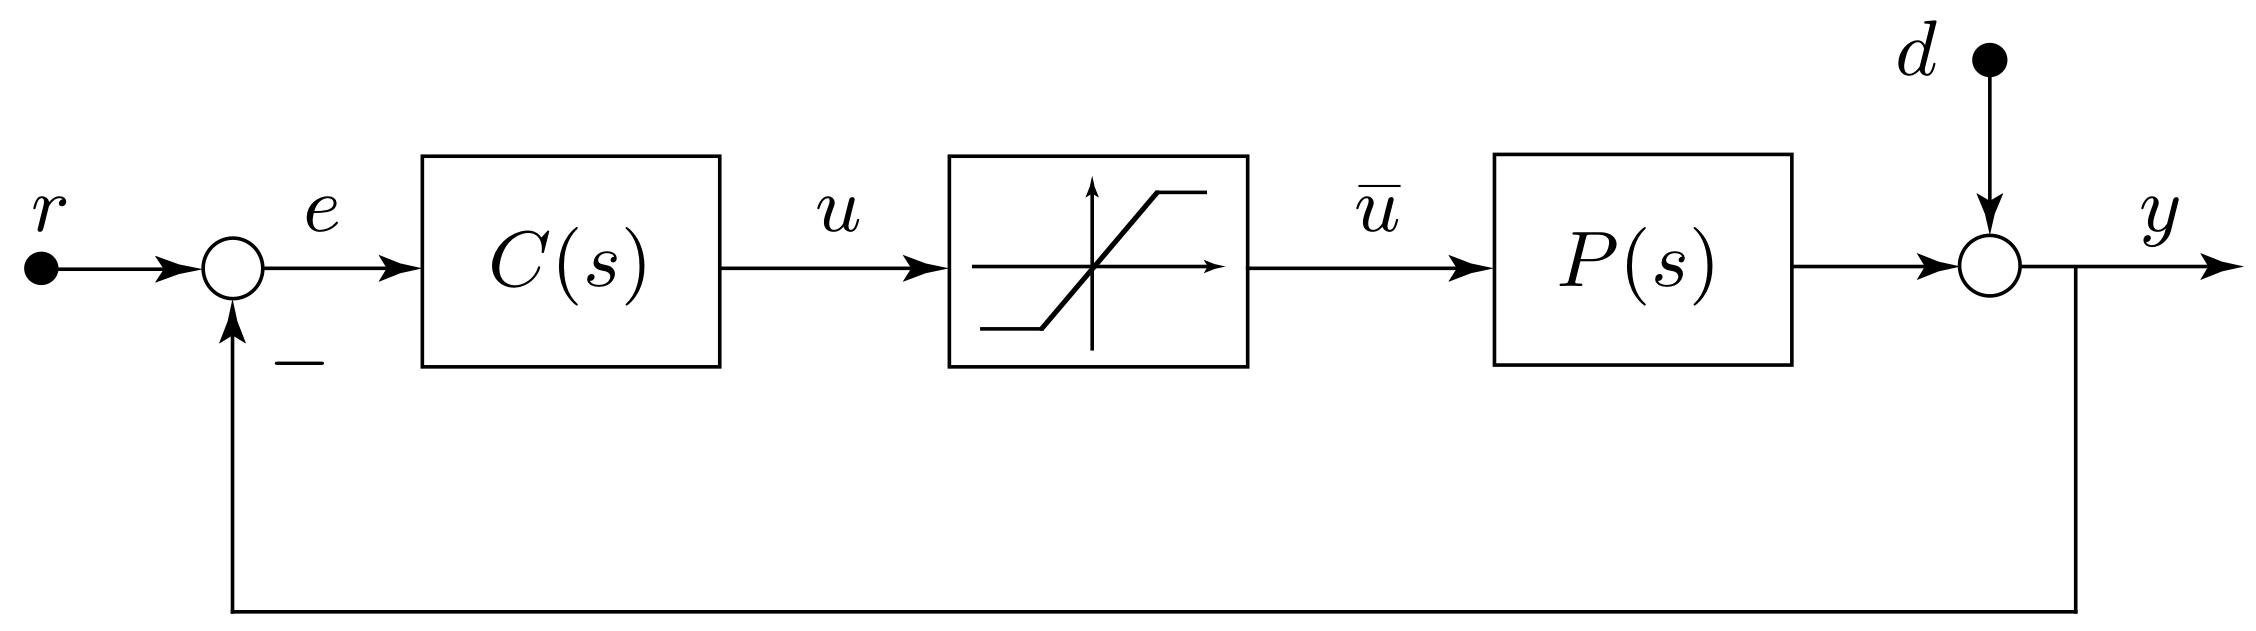
\includegraphics[width = 0.6\linewidth]{images/04/arw.jpeg}
    \end{figure}
    
    Wie kommt es zu Saturation? Da das System langsamer reagiert als man erwartet, haben Integratoren mehr Zeit um sich zu füllen. Sobald dann aber das Vorzeichen des Fehlers ändert Überschiesst der Regler zuerst das Ziel, da sich der Integrator zuerst wieder Entleeren muss um eine Änderung im Aktuatorsignal hervorzurufen. 
    
    \subsubsection{ARW/Bumpless Transfer}
        Um diese Saturation zu verhindern, wird der Integrator um ein \textit{Anti-Reset Windup} (ARW) erweitert, der das ``überfüllen" des Integrators verhindert. Dazu wird die differenz $q(t) = u(t) - \Bar{u}(t)$ vom Integrator abgezogen. Falls $u(t)$ nicht saturiert, ist $q(t)= 0$.
        
        Meist ist es sinvoll, nebst einem Automatischen Modus, einen Manuellen Modus für die Steuerung des Systems zu haben. Möchte man von einem Modus in den Anderen wechseln, so soll das so rebungslos/smooth wie möglich passieren, um Stösse auf das System zu verhindern. Dazu verwendet man den \textit{Bumpless Transfer}.
        
        \begin{figure}[H]
            \centering
            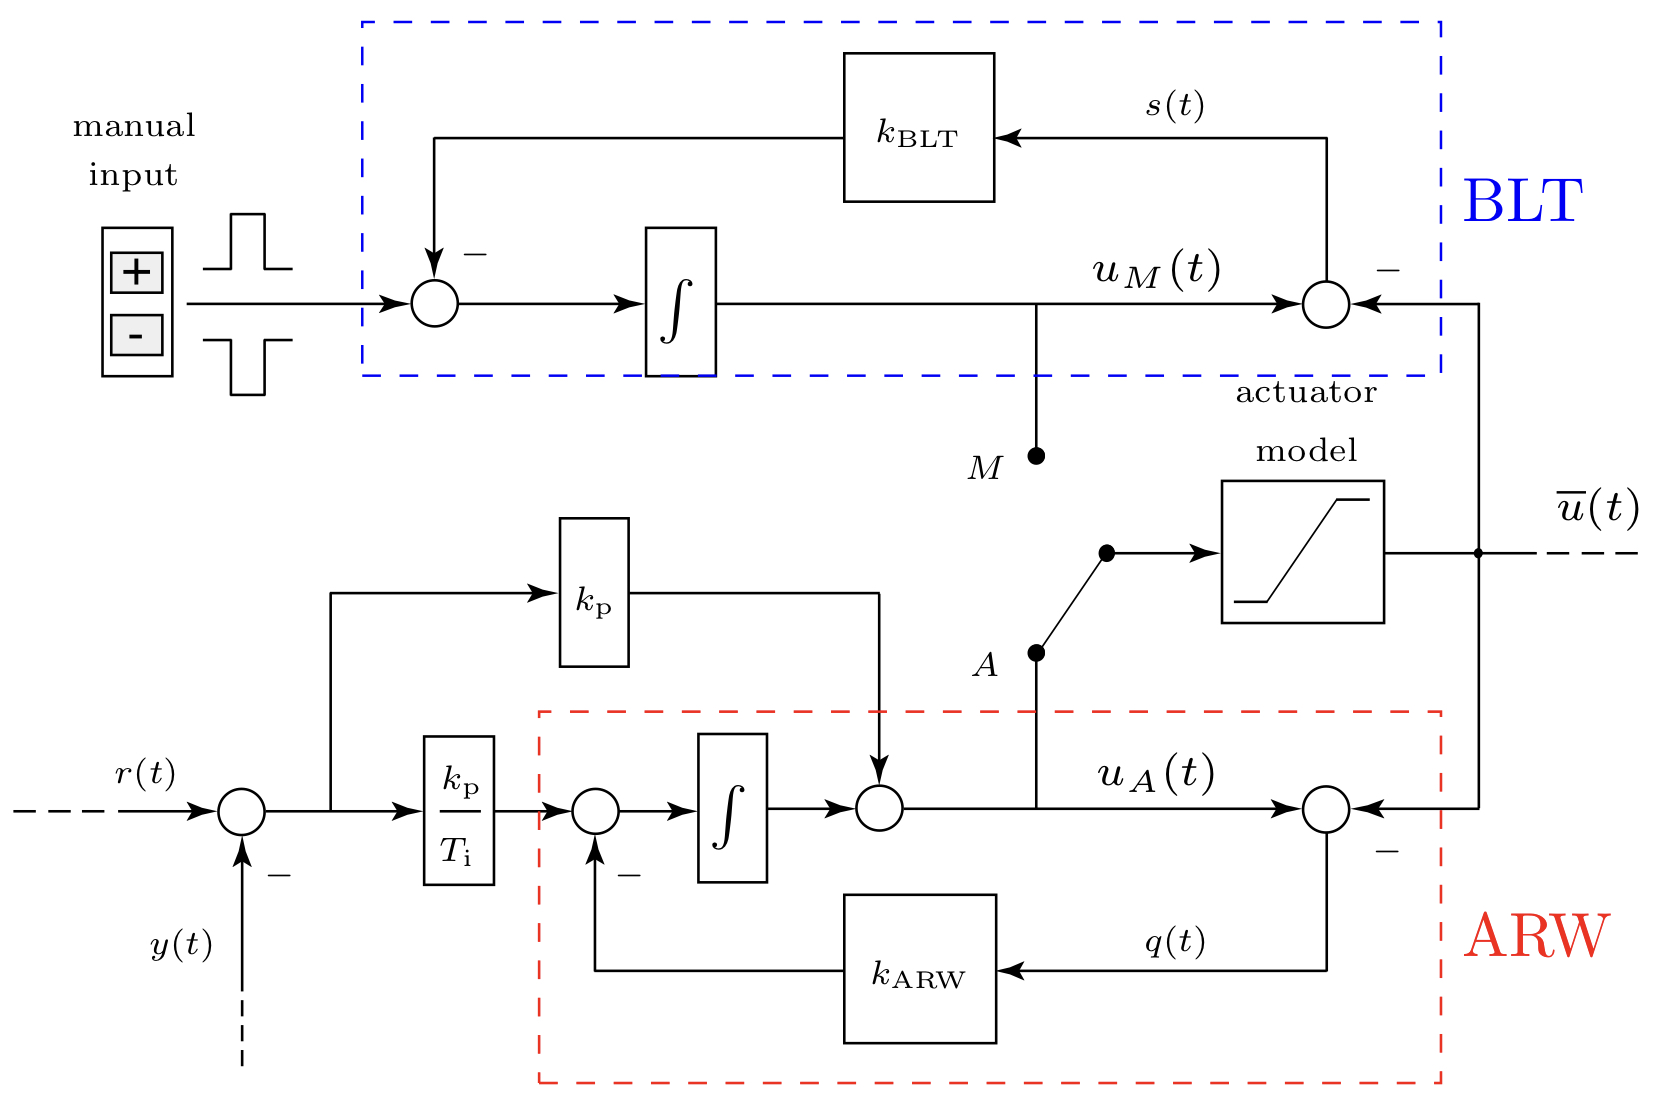
\includegraphics[width = 0.6\linewidth]{images/04/arw_bt.jpeg}
            \caption{Realisation von ARW und BLT}
        \end{figure}
        
    \subsubsection{Bsp}
        Für ein System wurde ein PI-Regler ausgelegt und das resultierende System wurde simuliert. Man stellt fest, dass die Perfomance ohne ARW schlechter ist, als mit ARW.
        
        \begin{figure}[H]
            \centering
            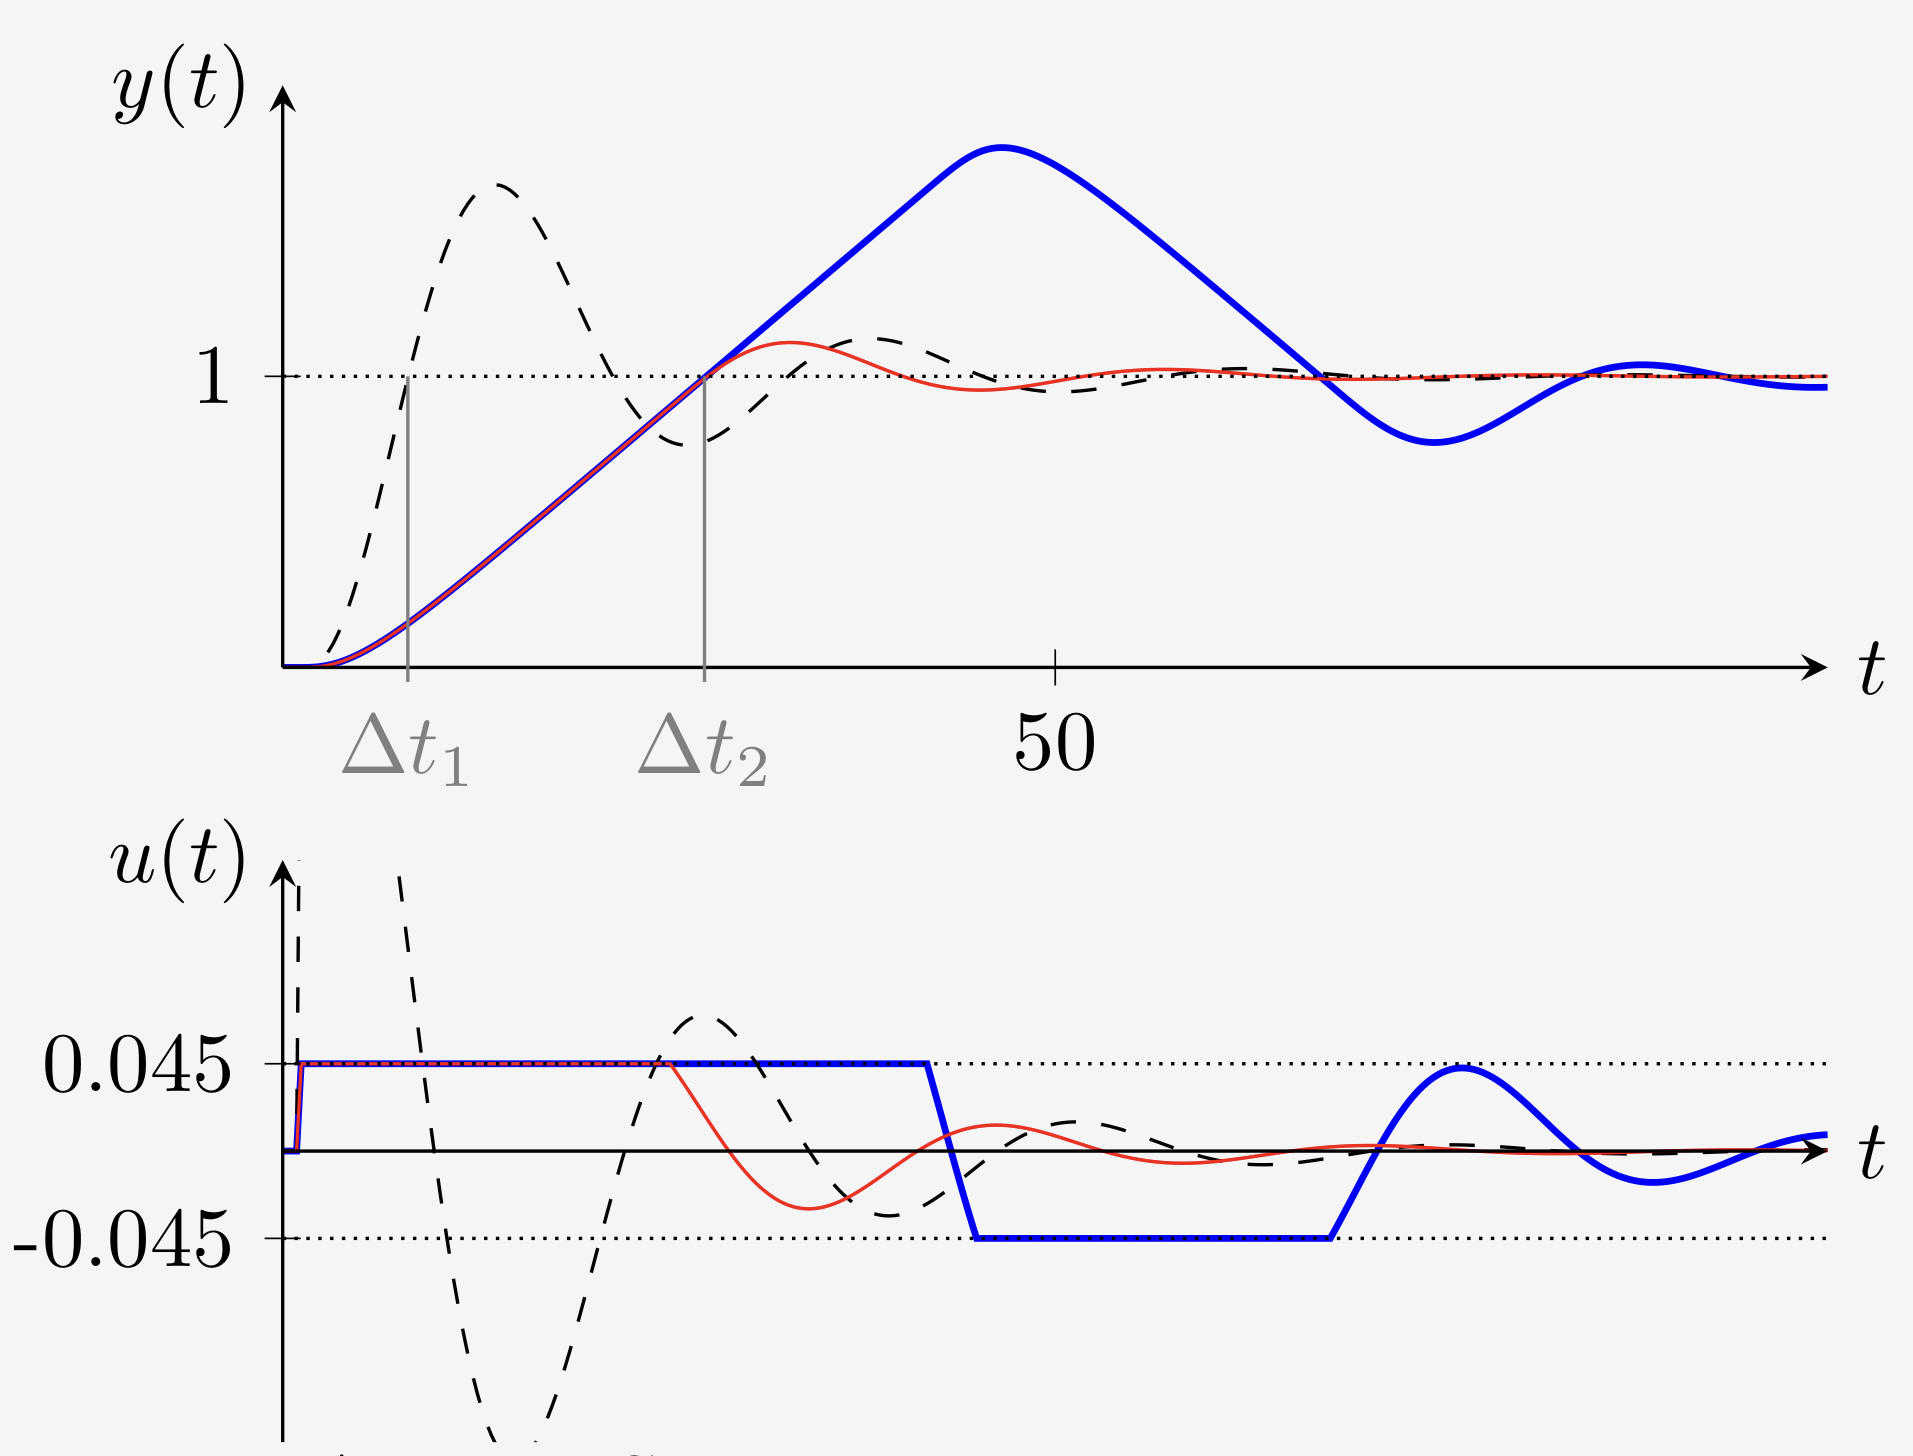
\includegraphics[width = 0.6\linewidth]{images/04/arw_bsp.jpeg}
            \caption{\textcolor{blue}{Blau: system ohne ARW}, \textcolor{red}{Rot: system mit ARW} und Dashed: Ideales System ohne Saturation}
        \end{figure}